%!TEX root = ../thesis.tex
\chapter{The one with cross entropy \label{ch:crossentropy}}

We can calculate...

\section{Entropy Rate}

Recall \autoref{def:entropyrate} of the entropy rate of a stochastic process, which while a useful theoretical tool, can be very difficult to compute. 
\todo{why is it hard to compute}

To overcome this, we seek a way to estimate the entropy of the process from a known sequence of data. In 1998 Kontoyianni et al. proved the convergence of a non-parametric entropy estimator in stationary processes~\cite{kontoyiannisNonparametricEntropyEstimation1998}.

\begin{definition}[Kontoyianni Entropy Rate] \label{def:kontoyianni}
	For a stochastic process $\mathcal{X} = \{X_i\}$, with a realisation of $n$ states and a finite alphabet,  the entropy rate can be estimated using,
		\begin{equation}\label{eq:estimate}
	H(\mathcal{X}) \approx\frac{|\mathcal{X}| \log |\mathcal{X}| }{\sum_{i=0}^n \Lambda_{i} },
	\end{equation}
	where $|\mathcal{X}|$ is the size of the alphabet and $\Lambda_{i}$ is the length of the shortest subsequence starting at position $i$ that does not appear as a contiguous subsequence in the previous $i$ symbols $X_{0}^{i}$. This can also be obtained by adding 1 to the longest match-length, 
	 \begin{equation}\label{eq:lambda}
	  \Lambda_{i}=1+\max \left\{l: X_{i}^{i+l}=X_{j}^{j+l}, 0 \leq j \leq N-i, 0 \leq l \leq N - i - j \right\}.
	 \end{equation}
\end{definition}


This idea of using matched subsequences of text draws from the original work by Lempel and Ziv~\cite{zivUniversalAlgorithmSequential1977} in compression algorithms based on coding schemes. These algorithms attempt to compress a sequence down into the smallest possible representation, which at perfect efficiency would be the entropy, $H$. However these universal coding algorithms have no universal rate of convergence \cite{shieldsUniversalRedundancyRates1993, shieldsUniversalRedundancyRates1995} and in practice other approaches are often employed, tailored to the specific application at hand.

The idea of an entropy estimator based on match lengths was originally put forward by Grassberger~\cite{grassbergerEstimatingInformationContent1989} and proved consistent for independent and identically distributed (i.i.d.) processes and mixing Markov chains~\cite{shieldsEntropyPrefixes1992}, stationary processes~\cite{kontoyiannisPrefixesEntropyRate1994} and more generally to random fields~\cite{quasEntropyEstimatorClass1999}.


Wyner and Ziv~\cite{wynerAsymptoticPropertiesEntropy1989} showed that for every ergodic process the match length $\Lambda_{n}$ grows like $\frac{\log{n}}{H}$ in probability. 

Extending from this notion Kontoyianni et al. showed the convergence of \autoref{eq:estimate} in stationary ergodic processes using the match-length $ \Lambda_{i}$. This match-length in \autoref{eq:lambda} can be seen as the length of the next phrase to be encoded in the sliding-window Lempel–Ziv algorithm.


\todo{talk more about how this match length works (diagram)}

\begin{figure}[hb]
	\centering
	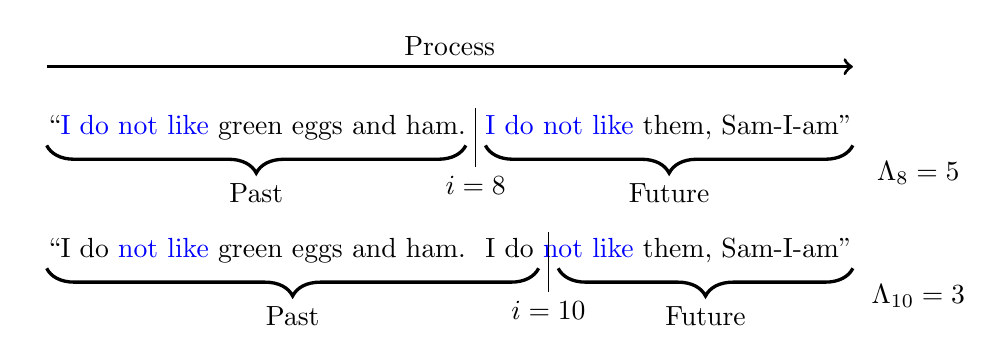
\begin{tikzpicture}
	% TOP ROW
	
	\node at (0,0) (a) {``{\color{blue}I do not like} green eggs and ham.};
	\node [right] at (a.east)  (b) {{\color{blue}I do not like} them, Sam-I-am''};
	
	\node [above] at (a.west) (westa){};
	\node [above] at (a.east) (easta) {};
	
	\node [above] at (b.west) (westb){};
	\node [above] at (b.east) (eastb) {};
	
	% Past brace
	\usetikzlibrary{decorations.pathreplacing}
	\draw [very thick, -, draw=black, decorate, decoration={brace,amplitude=10pt,mirror,raise=10pt} ] (westa) -- (easta)
	node[midway, below, yshift = -20pt] {Past} ;
	
	% Future
	\draw [very thick, -, draw=black, decorate, decoration={brace,amplitude=10pt,mirror,raise=10pt} ] (westb) -- (eastb)
	node[midway, below, yshift = -20pt] {Future} ;
	
	% Draw i line
	\draw (westb.north) -- ([yshift=-0.5cm]westb.south) node[below] {$i = 8$};
	
	\node [below right of = eastb] {$\Lambda_8 = 5$};
	
	% BOTTOM ROW
	
	\def\shift{0.8}
	
	
	\usetikzlibrary{positioning}
	\node [below = 1cm of a] (c) {``I do {\color{blue}not like} green eggs and ham.};
	\node [right] at (c.east)  (d) {I do {\color{blue}not like} them, Sam-I-am''};
	
	% Intermediary nodes
	\node [right = \shift cm of c.east] (shiftedceast) {};
	\node [right = \shift cm of d.west] (shifteddwest) {};
	
	\node [above] at (c.west) (westc){};
	\node [above] at (shiftedceast) (eastc) {};
	
	\node [above] at (shifteddwest) (westd){};
	\node [above] at (d.east) (eastd) {};
	
	% Past brace

	\draw [very thick, -, draw=black, decorate, decoration={brace,amplitude=10pt,mirror,raise=10pt} ] (westc) -- (eastc)
	node[midway, below, yshift = -20pt] {Past} ;
	
	% Future
	\draw [very thick, -, draw=black, decorate, decoration={brace,amplitude=10pt,mirror,raise=10pt} ] (westd) -- (eastd)
	node[midway, below, yshift = -20pt] {Future} ;
	
	% Draw i line
	\draw ([yshift=0.11cm]shifteddwest.north) -- ([yshift=-0.4cm]shifteddwest.south) node[below] {$i = 10$};
	
	\node [below right of = eastd] {$\Lambda_{10} = 3$};
	
	% Time Arrow
	\node [above = 0.4cm of westa]  (westtime) {};
	\node [above = 0.4cm of  eastb ](easttime) {};
	\draw [very thick, ->] (westtime) -- (easttime) node[midway, above] {Process} ;
	
	
	
	\end{tikzpicture}
	\caption{An example calculation of the match-length based $\Lambda_i$ applied to a line from Green Eggs and Ham by Doctor Seuss. {\color{blue} Blue text} is that which has been matched from past to the future. }
\end{figure}


Even before it's formalisation by Kontoyianni et al, similar estimators had appeared in the literature applied to experimental data to determine the entropy rates of processes~\cite{chenUsingDifficultyPrediction1993, chenFastPatternMatching1995, farachEntropyDNAAlgorithms1995, juolaWhatCanWe1997}.



\section{Assumptions of Entropy Rate Estimation}

\todo{A discussion and plots of entropy rate convergence}


\todo{A comparison with other entropy rates}


\begin{figure}[hb]
	\centering
	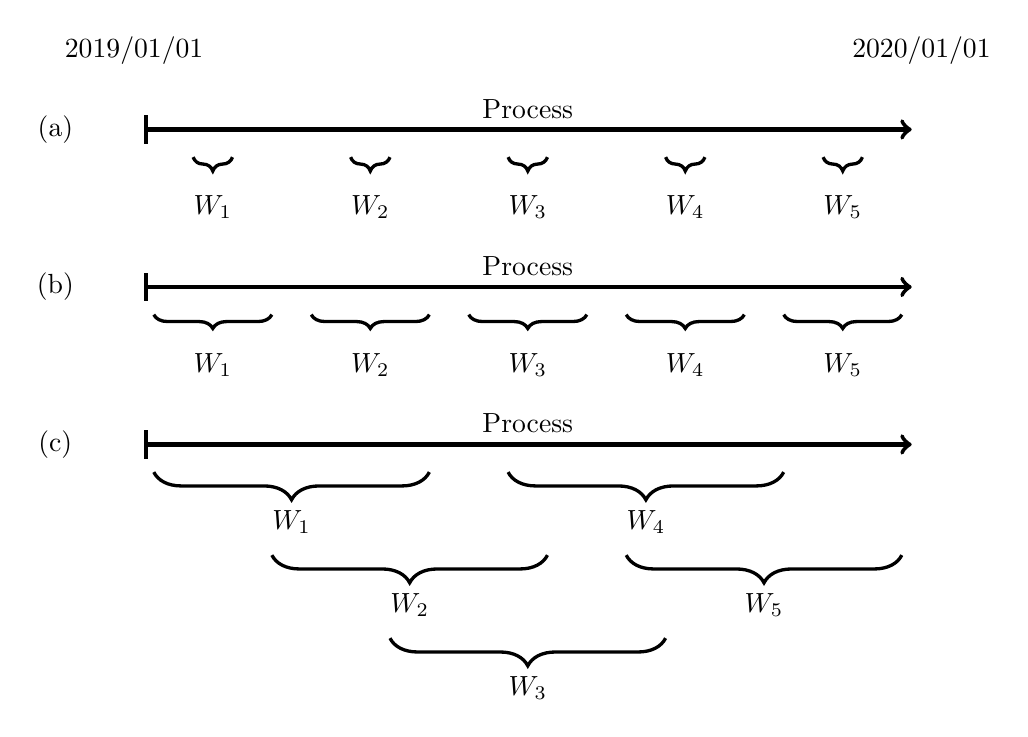
\begin{tikzpicture}
	
	\node at (-1,0) {(a)};
	
	% Time Arrow
	\node at (0,0) (lefttime) {};
	\node at (10,0) (righttime) {};
	\draw [ultra thick, |->] (lefttime) -- (righttime) node[midway, above] {Process} ;
	
	\node [above of = lefttime] {2019/01/01};
	\node [above of = righttime] {2020/01/01};
	
	\foreach \x [count=\i] in {0,2,4,6,8}{
		\draw [very thick, -, draw=black, decorate, decoration={brace,amplitude=5pt,mirror,raise=10pt} ] (0.75+\x, 0) -- (1.25+\x,0)
		node[midway, below, yshift = -20pt] {$W_\i$} ;
	}


	\node at (-1,-2) {(b)};
	
	% Time Arrow
	\node at (0,-2) (lefttime) {};
	\node at (10,-2) (righttime) {};
	\draw [ultra thick, |->] (lefttime) -- (righttime) node[midway, above] {Process};
	
	\foreach \x [count=\i] in {0,2,4,6,8}{
		\draw [very thick, -, draw=black, decorate, decoration={brace,amplitude=5pt,mirror,raise=10pt} ] (0.25+\x, -2) -- (1.75+\x,-2)
		node[midway, below, yshift = -20pt] {$W_\i$} ;
	}

	\node at (-1,-4) {(c)};
	
	% Time Arrow
	\node at (0,-4) (lefttime) {};
	\node at (10,-4) (righttime) {};
	\draw [ultra thick, |->] (lefttime) -- (righttime) node[midway, above] {Process};
	
	\draw [very thick, -, draw=black, decorate, decoration={brace,amplitude=10pt,mirror,raise=10 pt} ] (0.25, -4) -- (3.75,-4)
	node[midway, below, yshift = -20 pt] {$W_1$} ;
	
	\draw [very thick, -, draw=black, decorate, decoration={brace,amplitude=10pt,mirror,raise=40 pt} ] (1.75, -4) -- (5.25,-4)
	node[midway, below, yshift = -50 pt] {$W_2$} ;
	
	\draw [very thick, -, draw=black, decorate, decoration={brace,amplitude=10pt,mirror,raise=70 pt} ] (3.25, -4) -- (6.75,-4)
	node[midway, below, yshift = -80 pt] {$W_3$} ;
	
	\draw [very thick, -, draw=black, decorate, decoration={brace,amplitude=10pt,mirror,raise=10 pt} ] (4.75, -4) -- (8.25,-4)
	node[midway, below, yshift = -20 pt] {$W_4$} ;
	
	\draw [very thick, -, draw=black, decorate, decoration={brace,amplitude=10pt,mirror,raise=40 pt} ] (6.25, -4) -- (9.75,-4)
	node[midway, below, yshift = -50 pt] {$W_5$} ;
	

	\end{tikzpicture}
	\caption{\todo{}}
\end{figure}




\section{Cross Entropy Rate}

Similar to the extension of entropy to cross entropy in \autoref{def:crossentropy}, we can generalise our notion of Kontoyianni entropy rate in \autoref{def:kontoyianni} to a cross entropy rate.

\begin{definition}[Cross Entropy Rate]
	The cross entropy of a {\color{target} target process} $\mathcal{T}$ coded from a {\color{source} source process} $\mathcal{S}$ can be estimated,
	\begin{equation}
	\hat{H}(\mathcal{T} || \mathcal{S})=\frac{N_{\mathcal{T}} \log _{2} N_{\mathcal{S}}}{\sum_{i=1}^{N_{\mathcal{T}}} \Lambda_{i}(\mathcal{T}| \mathcal{S})}
	\end{equation}
	Where $\Lambda_{i}(\mathcal{T}| \mathcal{S})$ is given by the shortest subsequence starting at position $i$ in {\color{target}target} $\mathcal{T}$ that does not appear as a contiguous subsequence in the {\color{source}source} $\mathcal{S}$.
	\begin{equation}
	\Lambda_{i}(\mathcal{T}| \mathcal{S}) = \max \left\{l: T_i^{i+l}=S_{j}^{j+l}, 0 \leq j \leq N_{\mathcal{S}} \leq l \leq \min( N_{\mathcal{S}}- j , N_{\mathcal{T}}- i )\right\}
	\end{equation}
\end{definition}


% test what suffiently long means in complexity ( plot of complexity vs speed of convegence)




%
%	\begin{tikzpicture}
%
%%% TOP EVENTS
%
%\node at (-1, 0.5) {Source};
%
%% Events
%% Past Events
%\draw [thick, fill = blue!30!white] (0,0)  rectangle (10,1)  ;
%\foreach \x in {0, 0.8, 1.6, 3.2, 3.6, 5.2, 6, 8.4, 9.2}
%{
%	\fill[red!30!white] (\x ,0) rectangle ++(0.4,1);
%}
%
%% Future Events
%\draw [thick, fill = blue!60!white] (10,0) rectangle (14,1) ;
%\foreach \x in {10, 10.8, 12.8}
%{
%	\fill[red!60!white] (\x,0) rectangle ++(0.4,1);
%}
%
%% Redraw Main Rectangle
%\foreach \x in {0,...,34}
%{
%	\draw [very thin] (0.4*\x,0)  rectangle ++(0.4,1);
%}
%\draw [thick] (0,0) rectangle (14,1) ;
%
%
%
%%%ORANGE EVENTS
%
%\node at (-1, 0.5) {Source};
%
%% Events
%% Past Events
%\draw [thick, fill = blue!30!white] (0,0)  rectangle (10,1)  ;
%\foreach \x in {0, 0.8, 1.6, 3.2, 3.6, 5.2, 6, 8.4, 9.2}
%{
%	\fill[red!30!white] (\x ,0) rectangle ++(0.4,1);
%}
%
%% Future Events
%\draw [thick, fill = blue!60!white] (10,0) rectangle (14,1) ;
%\foreach \x in {10, 10.8, 12.8}
%{
%	\fill[red!60!white] (\x,0) rectangle ++(0.4,1);
%}
%
%% Redraw Main Rectangle
%\foreach \x in {0,...,34}
%{
%	\draw [very thin] (0.4*\x,0)  rectangle ++(0.4,1);
%}
%\draw [thick] (0,0) rectangle (14,1) ;
%
%
%
%% Future
%\draw [red!60!black, very thick, shorten >= -0.6pt]        (10,-2.5 ) -- (10,1.5);
%\draw [red!60!black, very thick, ->] (10,   1.5)  -- (13, 1.5)   node[midway, above] {Future} ;
%
%% Time Arrow
%\draw [very thick, ->] (0,2.5) -- (13,2.5) node[midway, above] {Time} ;
%
%% Past brace
%\usetikzlibrary{decorations.pathreplacing}
%\draw [very thick, -, draw=black, decorate, decoration={brace,amplitude=10pt,mirror,raise=4pt} ] (9.8,1) -- (0.2,1)
%node[midway, above, yshift = 14pt] {Past} ;
%
%\end{tikzpicture}


%old

%\resizebox{1\textwidth}{!}{
%	\begin{tikzpicture}
%	
%	%% TOP EVENTS
%	
%	\node at (-1, 0.5) {Source};
%	
%	% Events
%	% Past Events
%	\draw [thick, fill = blue!30!white] (0,0)  rectangle (10,1)  ;
%	\foreach \x in {0, 0.8, 1.6, 3.2, 3.6, 5.2, 6, 8.4, 9.2}
%	{
%		\fill[red!30!white] (\x ,0) rectangle ++(0.4,1);
%	}
%	
%	% Future Events
%	\draw [thick, fill = blue!60!white] (10,0) rectangle (14,1) ;
%	\foreach \x in {10, 10.8, 12.8}
%	{
%		\fill[red!60!white] (\x,0) rectangle ++(0.4,1);
%	}
%	
%	% Redraw Main Rectangle
%	\foreach \x in {0,...,34}
%	{
%		\draw [very thin] (0.4*\x,0)  rectangle ++(0.4,1);
%	}
%	\draw [thick] (0,0) rectangle (14,1) ;
%	
%	
%	
%	%%ORANGE EVENTS
%	
%	\node at (-1, 0.5) {Source};
%	
%	% Events
%	% Past Events
%	\draw [thick, fill = blue!30!white] (0,0)  rectangle (10,1)  ;
%	\foreach \x in {0, 0.8, 1.6, 3.2, 3.6, 5.2, 6, 8.4, 9.2}
%	{
%		\fill[red!30!white] (\x ,0) rectangle ++(0.4,1);
%	}
%	
%	% Future Events
%	\draw [thick, fill = blue!60!white] (10,0) rectangle (14,1) ;
%	\foreach \x in {10, 10.8, 12.8}
%	{
%		\fill[red!60!white] (\x,0) rectangle ++(0.4,1);
%	}
%	
%	% Redraw Main Rectangle
%	\foreach \x in {0,...,34}
%	{
%		\draw [very thin] (0.4*\x,0)  rectangle ++(0.4,1);
%	}
%	\draw [thick] (0,0) rectangle (14,1) ;
%	
%	
%	
%	% Future
%	\draw [red!60!black, very thick, shorten >= -0.6pt]        (10,-2.5 ) -- (10,1.5);
%	\draw [red!60!black, very thick, ->] (10,   1.5)  -- (13, 1.5)   node[midway, above] {Future} ;
%	
%	% Time Arrow
%	\draw [very thick, ->] (0,2.5) -- (13,2.5) node[midway, above] {Time} ;
%	
%	% Past brace
%	\usetikzlibrary{decorations.pathreplacing}
%	\draw [very thick, -, draw=black, decorate, decoration={brace,amplitude=10pt,mirror,raise=4pt} ] (9.8,1) -- (0.2,1)
%	node[midway, above, yshift = 14pt] {Past} ;
%	
%	\end{tikzpicture}
%}